\chapter{General Discussion}\thumbforchapter
\newpage

All cells in our body contain the exact same DNA, yet the cells in our liver express a completely different set of genes than the cells in our heart. Gene expression regulation is the mechanism that controls the activation and repression of genes in the genome. The spatial and temporal control of gene regulation is an essential part of (embryonic) development. Moreover, genes and their spatio-temporal expression patterns and regulation are exceptionally conserved between species.

In this thesis, we studied gene expression regulation from an evolutionary-developmental point of view. We first discuss three recommendations for gene regulatory network inference in development; multi-omics data, single-cell sequencing, and artificial neural nets (\textbf{chapter X}). Next, we present seq2science, a preprocessing workflow for functional genomics analysis (\textbf{chapter X}). We then continue with a description of how the definition of the phylotypic stage is ambiguous and how this ambiguity leads to the development of new statistical controls. Applying these new controls to previous studies finds flaws in the methodology and the subsequent interpretation of their results (\textbf{chapter X and Y}). Finally, in \textbf{Chapter Z} we present a novel method to infer transcription factor activity based on single-cell transcriptomic data. Here we present our final concluding remarks.

\section{The scientific dogma of the phylotypic stage}

\begin{shadequote}[c]{George Box}
All models are wrong, but some are useful.
\end{shadequote}

While historically the phylotypic stage has predominantly been examined and described through qualitative methods, the 21\textsuperscript{st} century started a paradigm shift towards a more quantitative and data-driven approach to understanding this phenomenon\cite{Chan2021}. The first notable quantitative investigation into the phylotypic stage was done by Bininda-Emonds \textit{et al.}, where they calculated temporal conservation as the order in which morphological embryonic features appear in vertebrates\cite{OlafRP2003}. However, it wasn't until the early 2010s that the field truly embraced quantitative methodologies with the simultaneous publication of two groundbreaking studies in Nature\cite{Kalinka2010, DomazetLoso2010}. In these works, Domazet-Lošo \textit{et al.} investigated the average developmental age of transcripts in \textit{D. rerio} and \textit{D. melanogaster}, whilst at the same time, Kalinka \textit{et al.} explored the temporal transcriptome similarities across different \textit{Drosophila} species. These molecular studies opened a new line of research to the quantitative basis of the phylotypic stage. The quantitative support for the phylotypic stage appears stronger and stronger with each new study. So strong, that we quickly forget all the nonconforming results.

The Transcriptome Age Index (TAI), as introduced by Domazet-Lošo \textit{et al.}, is a metric of the average evolutionary age of transcripts over time\cite{DomazetLoso2010}. In this study, evolutionary age is determined as the count of taxonomic branches that can be traced back to a gene. The central idea of the TAI is that temporal changes in the average transcript age provide insights into the degree of conservation during development. Domazet-Lošo \textit{et al.} found that both zebrafish and \textit{Drosophila} expressed the oldest transcriptome at their respective phylotypic stages and concluded that an old transcriptome marks the phylotypic phase. However, an independent re-analysis conducted by Piasecka \textit{et al.} raised some critical points about the methodology\cite{Piasecka2013}. Their investigation revealed that the TAI is heavily influenced by a relatively small subset of genes due to major differences in transcript levels per gene (transcriptomic data is notoriously heteroscedastic\cite{Rocke2001}). Log transforming the data, which is a standard processing step for this type of data, completely invalidates the results of the original study. One might expect such a dependency on data transformation to cast doubts on the reliability of the method. Surprisingly, the opposite appears to be true. The original study introducing the TAI has been cited 88 times between 2010 and 2013, but has been cited 359 times since Piasecka \textit{et al.}'s publication (covering the years 2014-2023). As it turns out, you can now analyze the data with and without transformation, and keep the results that reinforce your preferred hypothesis. A notable example of this is Wu \textit{et al.}'s study on Spiralian development\cite{Wu2019}. In their analysis of untransformed data for \textit{Crassostrea gigas}, \textit{Haliotis discus hannai}, and \textit{Perinereis aibuhitensis}, they claim to have found an inverse hourglass pattern of evolutionary conservation and speculate why spiralia have a different temporal selection pressure than other species. However, their supplementary data reveals a different pattern for \textit{Crassostrea gigas} after square root transformation, shifting from an inverse hourglass to a funnel shape. Remarkably, this crucial finding receives minimal attention in the study, with the authors merely stating that at least the transformed data does not show an hourglass-like pattern. Moreover, the transformed TAI of the other two species is not even shown, and upon closer inspection, it appears that the inverse hourglass pattern of \textit{Perinereis aibuhitensis} of untransformed data can simply be attributed to random noise. Where one should be careful with elaborate interpretations of this study, it has instead sparked an exchange among three influential evolutionary-developmental biologists - Pavel Tomanczak, Denis Duboule, and Andreas Hejnol - on Twitter (now X), about the universality of the hourglass model\cite{hejnoltwitter}. It is worth mentioning that Andreas Hejnol has authored two critical reviews about the methodology and design of previous studies that asserted the universality of the phylotypic stage\cite{Dunn2018,hejnol2016}.

The work of Barbara Piasecka, where she showed that the pattern of the TAI is caused by a subset of all genes was led by Marc Robinson-Rechavi. The main work of this study was not about the TAI, but about using a multitude of different metrics to estimate temporal evolutionary conservation. Their conclusion is that different metrics produce different results. In his personal blog, Marc Robinson-Rechavi concludes \say{First, that biology is complicated, and insisting on answers such as « the hourglass exists (and explains diverse data) » or « it doesn’t » may not be the best strategy. Second, that the technical details are very important}\cite{robinsonrechaviblog}. Marc Robinson-Rechavi's later career, however, appears to have diverged from his earlier conclusions. He has made assertive claims concerning the ortholog conjecture\cite{KryuchkovaMostacci2016} and the hourglass model of conservation\cite{Liu2020,Liu2021,marletaz2018}. A re-analysis by Casey Dunn, Andreas Hejnol, and others identified methodological issues with their analysis of the ortholog conjecture\cite{Dunn2018}, and in \textbf{chapter X} I discuss in detail the methodological problems of two of his studies related to the hourglass model.

In 2003, Bininda-Emonds \textit{et al.} conducted a quantitative study of the phylotypic stage, which was revisited seventeen years later by Gerardo A. Cordero \textit{et al}\cite{OlafRP2003, Cordero2020}. Both studies were about the quantitative temporal analysis of morphological characteristics. To the best of my knowledge, these are the only quantitative analyses of morphological characteristics with respect to the phylotypic stage. The initial findings of Bininda-Emonds \textit{et al}. revealed an unexpected inverse hourglass pattern in morphological rankings, a discovery that challenged the existing assumption of mid-development being the most conserved period. It took seventeen years for a follow-up study, that surprisingly showed precisely the opposite - an hourglass pattern. Unfortunately, Cordero \textit{et al.} only comment that the difference between these two studies \textit{could} be caused by a difference in morphological characteristics, methodology, and species used, without any further analysis of the differences. They were correct in their assessment however, as in \textbf{chapter X} I show through simulations that the inverse hourglass pattern of Bininda-Emonds \textit{et al.} is likely caused by the methodology's sensitivity to edge effects, and does not represent a biological signal.

In 2016, Levin \textit{et al.} introduced the transcriptomic inverse hourglass model as a potential method for distinguishing between different phyla\cite{Levin2016}. However, this study has been criticized by Casey Dunn and Andreas Hejnol for its lack of a within-phylum control\cite{hejnol2016} and incorrect statistical methods\cite{Dunn2018}. Given the ambitious claim of a "universal" phylotypic stage characterized by a high similarity within phyla but a low similarity between phyla, it is somewhat perplexing that these criticisms have not yet been addressed by Levin \textit{et al}. What makes the situation even more confusing is that another group of evolutionary developmental biologists compared the embryonic development of deuterostomes and the chordate amphioxus - a between-phyla comparison. Astonishingly, they uncovered an hourglass-like pattern\cite{PerezPosada2022}, directly contradicting Levin \textit{et al.}'s inverse hourglass model, but do not comment on this. In \textbf{Chapter XXX}, I present evidence that the transcriptomic inverse hourglass is a statistical artifact resulting from normalization rather than an accurate representation of temporal conservation. 

Yoav Mayshar \textit{et al.} studied the phylotypic stage and the hourglass model from a single-cell point of view\cite{Mayshar2023}. Their research involved a comparative analysis of cell type proportions during the development of rabbit and mouse embryos. However, in \textbf{Chapter X}, I show that both the rabbit time series as well as the mouse time series exhibit discontinuous patterns. These discontinuities influence the temporal correlations between the two species. Without a better distributed temporal sampling, a direct comparison with this data in relation to temporal conservation is not possible. Moreover, when there is a mid-developmental transition between two time series, pairwise comparisons between these two time series are visually similar to an hourglass. Thus confusingly, when comparing two time series, if the data visualization shows an hourglass-like pattern, this represents the inverse hourglass model. It seems that Mayshar \textit{et al.} fell for this pitfall, as they perceive their mid-developmental transition as confirming the traditional hourglass model. Perhaps even more surprising, is that no one cared to correct their misinterpretation when they published their preprint on Biorxiv and that the reviewers of Cell, one of the most prestigious journals, failed to notice it.

\begin{figure}
    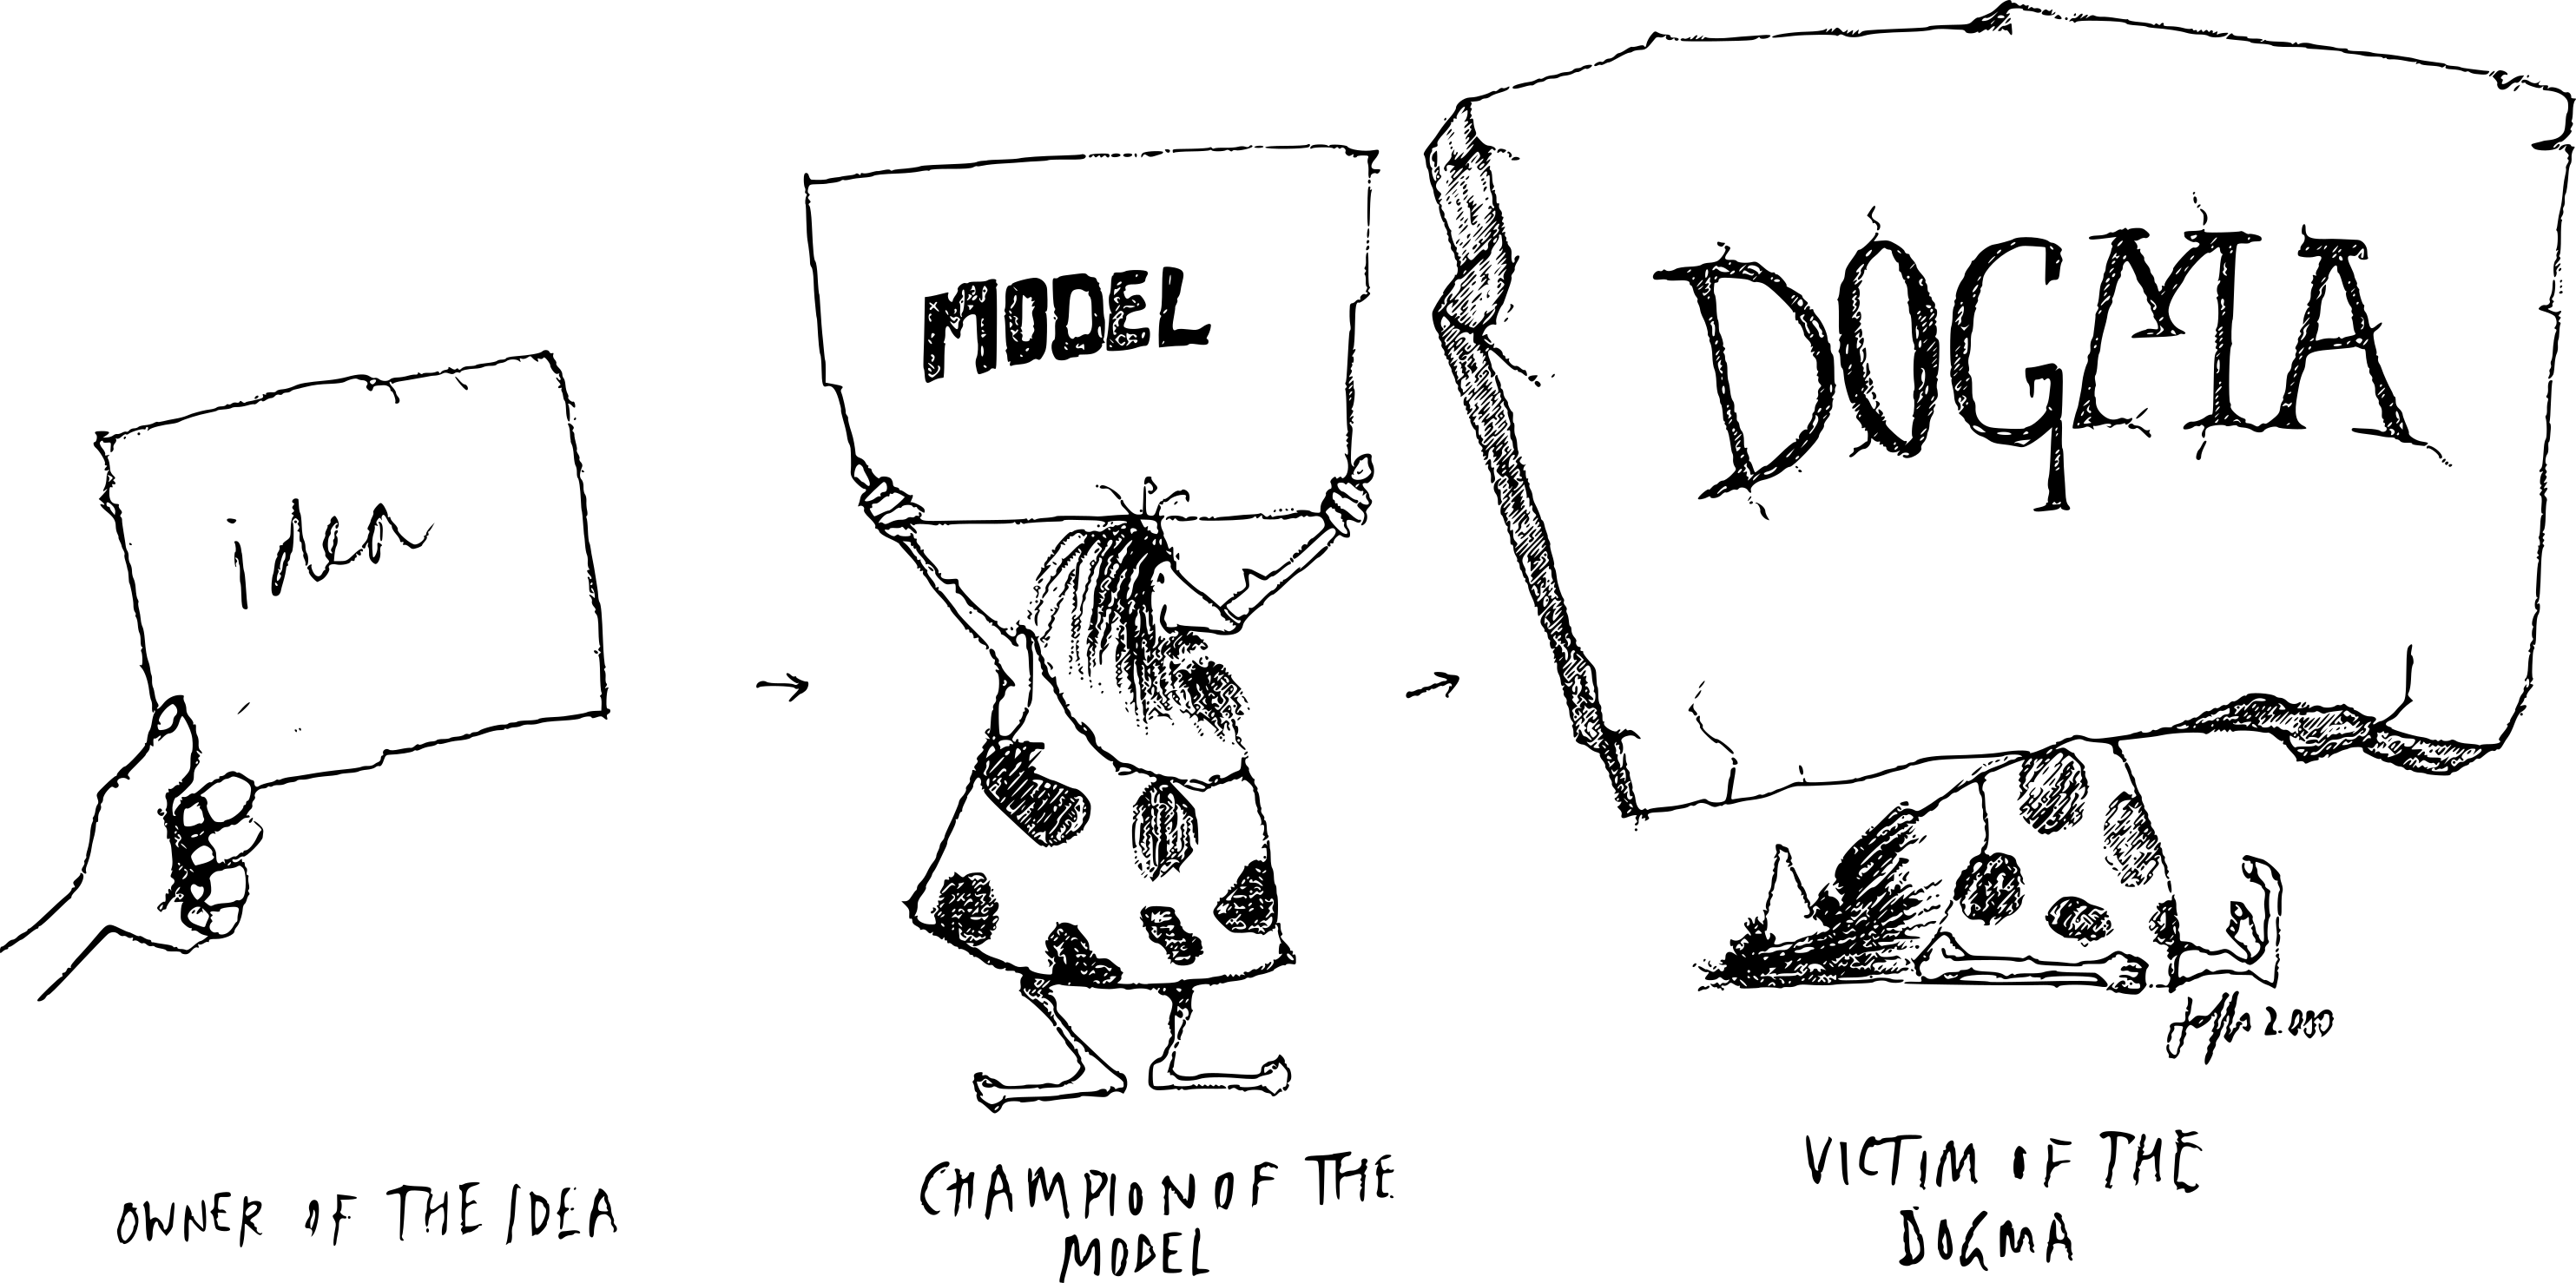
\includegraphics[width=\linewidth]{ch.discussion/imgs/dogma.png}
    \caption{\textbf{The phylotypic stage as a (crushing) scientific dogma?} \cite{Caveman2000}.}
    \label{fig:dogma}
\end{figure}

These examples highlight the dogmatic belief in the (non)existence of a phylotypic stage, and a reluctance to sincerely interact with each other's works. On top of that, in \textbf{chapter X and Y}, I discuss the methodological issues in comparative analyses concerning the phylotypic stage. The root problem is that the phylotypic stage and its related models are ill-defined, and as a consequence, there is a concerning lack of appropriate (statistical) controls in these studies. Is temporal conservation in these models present in comparisons within and between phyla? And is temporal conservation already observable when comparing a species against itself? By systematically addressing these ambiguities in previous studies through within-species, between-species, and between-phyla comparisons I show examples where the conclusions are not supported by the data. To summarize my main findings:
\begin{itemize}
    \item The transcriptomic hourglass-like pattern between zebrafish and frogs\cite{marletaz2018} can be explained by within-species correlations alone.
    \item The transcriptomic between-phyla inverse hourglass pattern\cite{Levin2016} is a statistical artifact and can be reproduced by simulated data with no specific temporal conservation.
    \item The pattern of cell type proportion similarity between rabbits and mice\cite{Mayshar2023} can be explained by discontinuous temporal sampling.
    \item The \textit{Drosophila} enhancer conservation re-analysis results in a "mid-developmental" stage of maximum similarity, albeit at a different point than found by the original authors. Moreover, in \textbf{Chapter X} I highlight additional problems with the binarization of enhancers, and as such I do not endorse this methodology.
    \item  The morphological within-phylum inverse hourglass pattern is caused by edge effects and can be reproduced by simulated data with no specific temporal conservation.
\end{itemize}
\noindent
The null model for evolutionary embryonic development would be that there is no specific stage of higher or lower temporal conservation. Altogether, I have found little evidence to reject the null hypothesis of constant temporal conservation based on quantitative data, and thus see no reason to believe in a (molecular) phylotypic stage.

Moreover, in \textbf{Chapter X} I discuss further ambiguities in the models of the phylotypic stage. If a molecular phylotypic stage would exist, which features are expected to be conserved and which are not? The original observation that vertebrate embryos, perhaps, look more like each other \textit{externally} at certain points in development, says little about the whole-embryo molecular basis for it. While the morphological observations of Haeckel are almost 200 years old, there have been only two quantitative studies about the morphological phylotypic stage, and these two studies are in direct contradiction with each other. Instead, there appears to be a pursuit to find new (quantitative) methodologies that produce a more straight-forward confirmation of the existence of the phylotypic stage, such as embryonic lethality\cite{Uchida2018}, morphology\cite{OlafRP2003,Cordero2020}, DNA sequence conservation\cite{Piasecka2013,Quint2012,Liu2021} and activation order\cite{Uesaka2019}, cell type proportion\cite{Mayshar2023}, and whole-transcriptome similarity\cite{Piasecka2013,Irie2011,marletaz2018,Liu2020,Leong2021,PerezPosada2022,Kalinka2010}, with little sincere effort to integrate these results across studies. Of these methodologies, the whole-embryo transcriptome has become the most popular method to asses quantitative similarity. The implicit justification for this is that the transcriptome is an unbiased way to study genes during development. Yet, the more cynical interpretation is that whole-embryo transcriptomic studies are the most confirming of our prior beliefs about the phylotypic stage. Even assuming the phylotypic stage exists, why would we expect to be able to measure such a complex phenomenon with such crude methods as observational studies and whole embryo sequencing? 

Throughout the course of scientific history, certain theories, such as taxonomic phyla and the phylotypic stage, have evolved from initial concepts into widely accepted truths, creating a demand for a molecular explanation along the way. However, a fundamental issue arises from the loose and ambiguous definitions on which these theories are based, leading to their lack of predictive power and falsifiability, rendering them, by Popperian standards, non-scientific in nature. For instance, the concept of phyla hinges on the notion that animals sharing a common basic body plan are part of the same phylum, yet paradoxically, the basic body plan is defined as the morphological characteristics shared by all animals within the same phyla\cite{BUDD2000,scholtz2004bauplane}. The definition of the phylotypic stage is similarly ambiguous. Historically, the pharyngula stage\cite{BALLARD1981}, early somite embryo\cite{Alberch1993}, and the tail bud stage \cite{Slack1993} have all been proposed as the vertebrate phylotypic stage. In quantitative studies, the choice of definition in turn depends on which stage exhibits the highest quantitative conservation. Consequently, the pharyngula \cite{Irie2011,marletaz2018}, the early somite embryo \cite{DomazetLoso2010}, or simply the stage(s) with the highest conservation metric\cite{Kalinka2010,Cordero2020} have all been identified as phylotypic stages. Our current approach to studying the phylotypic stage, where we selectively include definitions and ignore nonconforming results, is not only wrong but also not useful.

\section{Inferring gene regulatory networks}

Gene regulatory network inference is .... Understanding the interactions between transcription factors and genes helps with gaining a fundamental understanding of cellular processes, which ultimately can help with biomarker discovery and drug target identification. It has become a standard analysis step in most (single-cell) studies, however, the field seems to dismiss the fact that the inferred networks perform barely any better than random networks\cite{McCalla_2021,Chen_2018,Pratapa_2020}. Similarly, of all the clinical studies reaching phase I, almost 50\% fail because a drug is not efficient\cite{Sun2022}, \textbf{but it is unclear what percentage is based on functional genomics}. It is imperative that we improve GRN inference. In \textbf{Chapter XYZ} we discuss three improvements over "traditional" gene regulatory network inference; the inclusion of multi-omics data, single-cell sequencing, and artificial neural networks.

The first recommendation we suggest is the inclusion of multiple sequencing modalities. Historically gene regulatory networks have mainly been inferred based on transcriptomic data alone. Apart from the issue that these networks perform poorly\cite{McCalla_2021,Chen_2018,Pratapa_2020}, there is the fundamental issue of using transcripts both as input and as output in these models. Transcript abundance is the result of transcriptional regulation and degradation. Transcripts, however, are typically not responsible for signal transduction, chromatin remodeling, translation, and transcriptional regulation and degradation, but somehow when modeling these networks they are used as such. The protein product synthesized from these transcripts is responsible and is assumed to correlate closely with transcript abundance. The correlation coefficient between transcript and protein however ranges between 0.4-0.3\cite{Fortelny2017,Franks2017}, with transcript abundance thus approximately explaining only between 0.16-0.09 of the variance of protein abundance. High-throughput proteomics is more costly and lacks the accuracy of sequencing data, with single-cell proteomics lagging behind single-cell sequencing\cite{Bennett2023}. This in turn has led to the adoption of including genomic methods like genome accessibility and histone modifications as extra measurements for transcriptional regulation\cite{Xu_2020,Kamal_2021,Aibar_2017}, which in turn improves the performance of these models. Ideally, future GRN inference methods include genomic, transcriptomic, and proteomic information, and using only transcriptomic data was perhaps in hindsight a naive endeavor.

\begin{figure}[H]
    \centering
    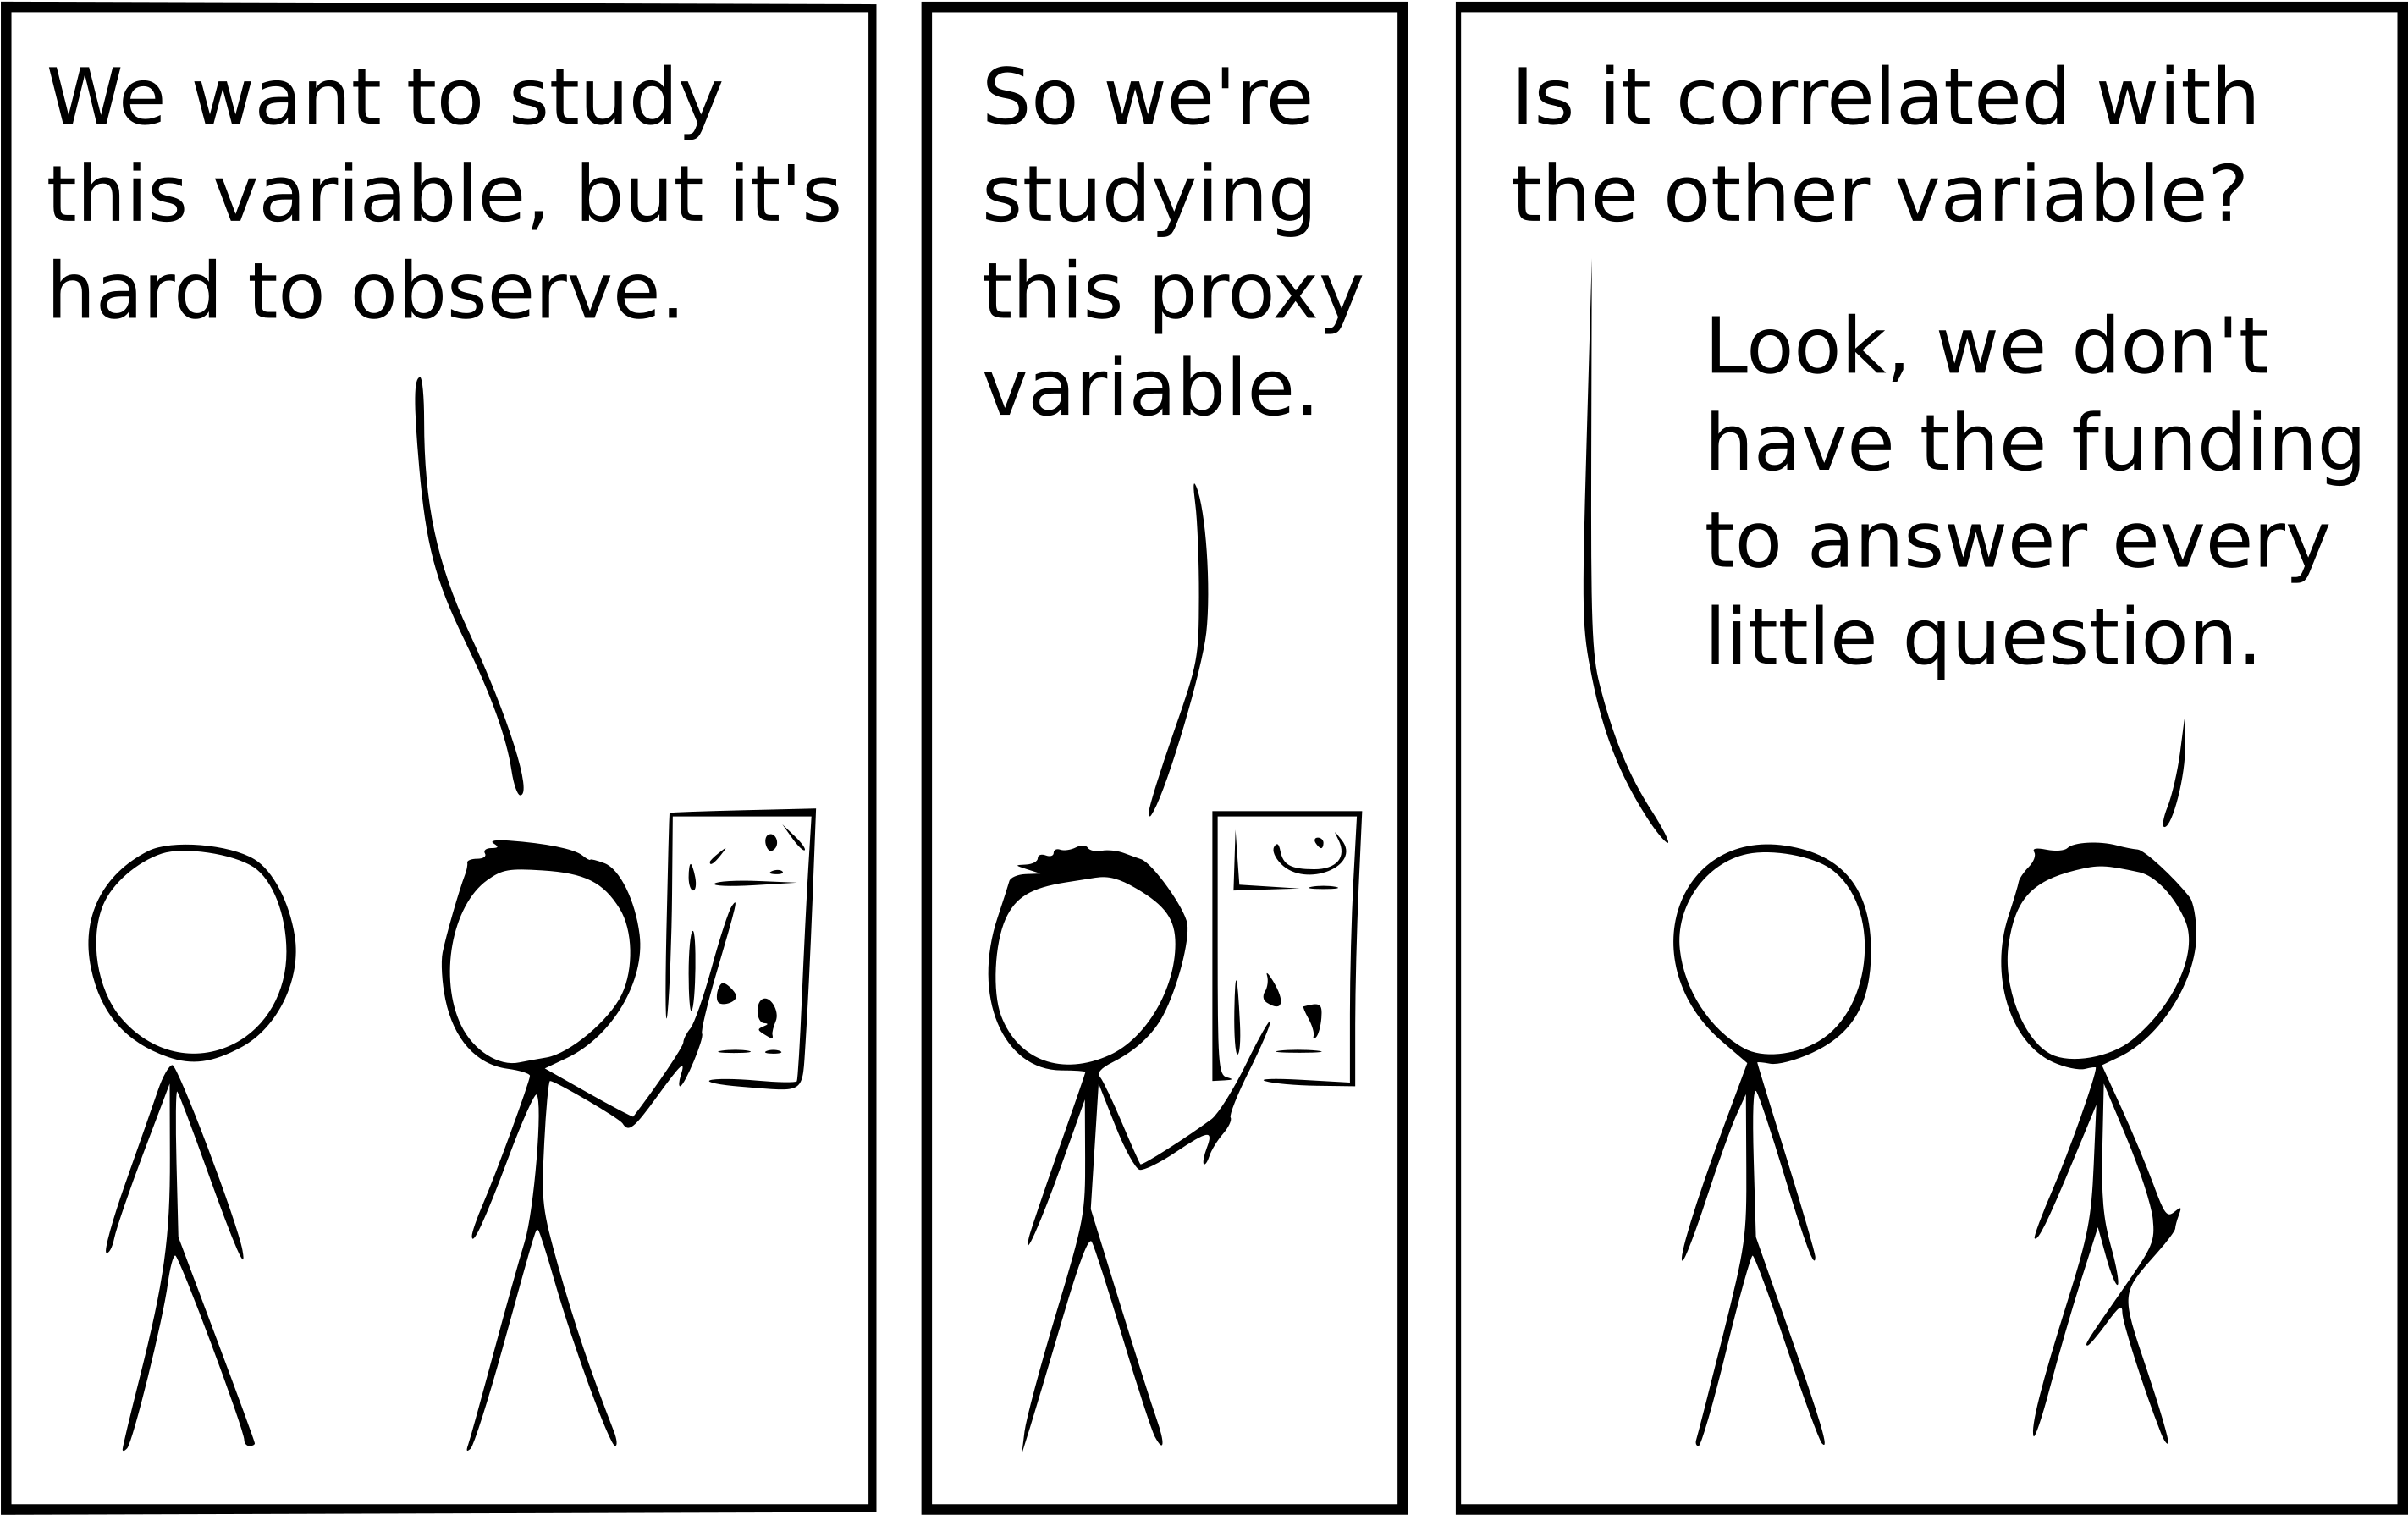
\includegraphics[width=0.7\linewidth]{ch.discussion/imgs/xkcd_proxy.png}
    \caption{\textbf{RNA-seq is used as a proxy for both the amount of gene regulation and protein abundance when inferring gene regulatory networks}. The correlation between transcripts and protein is however very weak. \textbf{xkcd}. URL: https://xkcd.com/2652}
    \label{fig:xkcd_proxy}
\end{figure}

The second recommendation we offer is the use of single-cell data. Single-cell sequencing is important because it separates the different signals present in tissues. Moreover, by separating cells in samples it is possible to order them on a fine-grained (pseudo)time\cite{Saelens2019}, increasing the detail and potential computational approaches of analyses. The analysis of single-cell data however has turned out to be problematic with major issues of batch effects \cite{Tran2020,Haghverdi2018,Lhnemann2020} and sparsity\cite{Lhnemann2020,Bouland2023}. Furthermore, gene regulatory networks inference methods specific for single-cell transcriptomic data are actually not more accurate than their "bulk" counterparts\cite{Chen_2018}. So whilst single-cell sequencing is important, in practice the real benefits are still to be gained.

The final recommendation we make is the use of artificial neural networks, which is a recommendation I would like to redefine here. Artificial neural networks are a powerful method capable of learning any (continuous) relationship in the data\cite{Cybenko_1989,Hornik_1989}. One of the reasons we recommended the use of ANNs is because they can incorporate and train on data over multiple conditions. This means that the networks that come out of these models are "universal", as in that they can be based on data of for example heart, liver, eye, and skin. As long as enough data is used we can expect these learned networks to be able to extrapolate to new unseen conditions. This makes these types of networks powerful methods for hypothesis generation, especially compared to the usual approach of inferring gene regulatory networks on the difference between two conditions. However, ANNs are not the only type of method that can produce "universal" networks. For instance, mechanistic models exist that model 

However, the underlying idea of using ANNs is that they can be trained on many sources of data, thus becoming a sort of "universal" gene regulatory network. As there is only a single set of instructions, DNA, we should model our GRNs on this idea. 
ANNs is perhaps the wrong term here, as it should not be about the tool. But about the idea. The idea is universal neural networks. As there is only a single set of instructions (DNA), we should model gene networks based on this idea. We should not try to infer the differential network between two cell states. Instead, we should strive to make a single network for all cell states. Fundamentally, this is more correct, and a network trained on the difference between two cell types is probably not capable of making predictions about perturbations. Moreover, making universal networks has the enormous advantage of having more data to train. (see schreiber avacodo). However, this needs to be done carefully, as there is stuff conserved, and data leakage between species would easily occur. Inflating the performance.

In \textbf{Chapter XX} I introduce the computational tool scepia. Scepia is based on single-cell and multi-omics data, but the inferred network simple. Also, we have absolutely no clue what makes scepia work and what does not. A proper parameter sweep would be really nice, something like in https://www.biorxiv.org/content/10.1101/2023.11.09.563812v1. Some design choices are very important, and others don't matter much.

And, finally

Finally, perhaps it is important to ask ourselves what is ultimately the goal of these GRNs? Do we care about having a map with all the arrows? Because the current correlation-based networks won't help us with differentiation networks. 

Calls for a more formal approach to gene regulatory network inference are old. Can a biologist fix a broken radio\cite{Lazebnik2002}. Twenty years later, the analogy unfortunately still holds true.

\section{The technical debt of bioinformatics}

Biological systems are inherently complex, which in turn makes their (bioinformatics) analysis complicated. The complexity of these analyses is worsened by the continuous addition of new technologies and insights. However, unnecessarily adding to this complexity is the use of outdated and idiosyncratic software and file formats. This in turn leads bioinformaticians to more easily make mistakes and do duplicate work. In software development, this problem is known as "technical debt". Technical debt is analogous to financial debt, where you borrow money and must eventually pay it back, including interest. I believe that in the field of bioinformatics, the technical debt has become so large that it has become prohibitive for analyses.

The most common file formats in bioinformatics were designed in the 90s and 00s, reflecting the tools of their time. Perl and awk were popular languages for bioinformatics, and for this reason, file formats are mostly plain text and line-based. The sam, bam, bed, gff, and vcf file formats all specify genomic features and their location, and are a great example of ill-thought-through design. The bam- and bed-format are zero-indexed\cite{Li2009}, whilst the sam-, gff-, and vcf-format are one-indexed\cite{Li2009,Danecek2011}. This makes one-off errors between these formats extremely easy and incurs significant development time for anyone working with these formats. Moreover, as our understanding and analyses got more complex, it became necessary to express more complex relationships between features within the file. This has led to a multitude of similar but incompatible gff versions and formats. The addition of these more complex relationships in gff files has made the format less suitable to be parsed line-by-line, which the format was originally designed for. An illustrative example highlighting the issues with positional formats is a tweet by Lior Pachter, where he asked if there is a citation for the gtf format. The most popular response covered the collective frustration of the field, stating \say{Ain’t no one gonna take responsibility for that mess}.
% https://twitter.com/lpachter/status/1719492098771300536

Another example of an outdated file format in bioinformatics is the fasta file format which\cite{Lipman1985}. The fasta file format, which was developed in 1985, is a text-based format that represents nucleotide sequences or amino acid sequences, in which nucleotides and amino acids are represented using single-letter IUPAC codes. Its age initially shows because lines are typically split over 80 characters, as that was the maximum screen width of the past. The true problem with the fasta format is, however, that it can not naturally represent uncertainty at genomic locations. Single nucleotide polymorphisms are defined by their IUPAC codes, but uncertainties longer than a single nucleotide can not be naturally represented. The solution for this problem has been to append alternative sequences to the fasta. These sequences can then selectively be used in the downstream analysis. However, bwa mem(2)\cite{bwamem,bwamem2}, and Illumina Dragen are the only genomic aligners that currently support this, even though alternative regions have been added to the human genome since 2013. A switch to a graph-based genome format\cite{Li2020} is obvious and seems unavoidable, but has somehow been postponed by the bioinformatics community. More confusing than the outdated file format is the slow adoption of updated genome assemblies. For example, in 2023, Google Scholar identified 7,630 publications that utilized the older hg19 or grch37 genome assemblies (released in 2009), while there were only 8,960 publications that used the newer hg38 or grch38 assemblies (released in 2013). Notably, the T2T-CHM13 assembly (released in 2022) has only received 222 citations so far in 2023. A better genome assembly, not surprisingly, results in more accurate clinical discoveries \cite{Aganezov2022}. Ultimately, the slow adoption of updated genomes by the community and the limitations of the fasta format inhibit discoveries in the field of bioinformatics.

\textbf{A project with significant technical debt is the Sequencing Read Archive (SRA), which shares enormous amounts of public sequencing data.} The SRA has been essential for my doctoral studies, as I have relied solely on public data. For \textbf{chapter XXX}, we aimed to download all available human H3K27ac data (+/- 12,000 samples) from the SRA as a reference database. Processing these samples meant that we had to download 20TB from the SRA and spent approximately 300,000 CPU hours processing them on Cartesius, costing roughly €1,000 for the SRA\cite{amazon}, €9,000 for Cartesius, and emitting nearly one tonne of CO2\cite{CO2}. In the analysis that followed, however, it turned out that obtaining sample annotations, such as tissue or cell type, is challenging due to the lack of standardized metadata on the SRA. Even though third-party tools like MetaSRA\cite{Bernstein2017}, and PredictMEE\cite{Klie2021} have been developed to automatically infer this metadata, they did not manage to resolve my issues. In the end, we decided to discard the experiment, wasting an enormous amount of resources.

Not only is the SRA missing crucial metadata, but their sra-tools, a toolkit for downloading sequencing data, are also particularly difficult to use. As a consequence, many alternative tools have been developed for downloading data from the SRA, such as the SRA-explorer\cite{sraexplorer}, pysradb\cite{pysradb}, FetchFastQ\cite{galvez2022metadata}, nf-core/fetchngs\cite{fetchngs}, parallel-fastq-dump\cite{parallelfastq}, and finally our download-fastq workflow of seq2science\cite{seq2science} (see \textbf{chapter XXX}). The technical debt of the sra-tools, as in a poor sra-tools implementation, results in additional and unnecessary work, wasting the time and resources of others. Similarly, the submission of new sequencing data is notoriously complicated, causing people to make mistakes, which even leads to others developing tools to streamline this process\cite{Quiones2020}. During my doctoral studies, I have come across many instances of data being mislabeled or missing, consuming a considerable amount of my time, presumably because of the difficult upload process.

A similar case where the technical debt of one group extends to others is MACS2. MACS2 is one of the most popular tools in bioinformatics and is used to discover enriched regions in the genome, and has been cited more than 14,000 times\cite{Zhang2008}. MACS2 has been continuously developed since 2008, and its developers should get credit for this effort. Nevertheless, MACS2 is a particularly poorly designed and unoptimized software tool. The recommended way to use MACS2 in the case of ATAC-seq discards all mates from paired-end data, effectively removing half of the cleavage information\cite{Gaspar2018}. This can be overcome by removing the mate tag of reads after alignment, or by converting the bam alignment file to a bed and using that as input. Most users are however not aware of this unexpected implementation, resulting in a suboptimal set of called peaks. A similarly surprising design choice is that MACS2 did not support more than two replicates for over 10 years (until I added it in a pull request). As a practically identical, but better alternative to MACS2, Genrich has been developed by an independent group\cite{genrich}. 

Finally, the quickest developing part of molecular analyses currently is the field of single-cell analyses. As a consequence, the most technical debt is taken in these parts. Single-cell tools are usually implemented poorly, taking days to run and requiring enormous amounts of memory. The usual solution to this problem is not to improve the software implementation, but instead to increase the hardware capabilities. For instance, an ex-colleague of mine requested a massive 4TB of RAM for his computer at his new position. A particularly painful point of technical debt in the single-cell field is the implementation of the log fold change calculation of Seurat. Seurat calculates the log of the means (as opposed to the mean of the logs), which makes it sensitive to outliers and this implementation should be corrected. This results in vastly different outcomes depending on whether one used Seurat or any alternative tool such as Scanpy for their analysis. The bug was reported in November 2022, got an incomplete fix in March 2023, and as yet has not been fixed (https://github.com/satijalab/seurat/issues/6654). Seurat has been cited 7,699 times\cite{Butler2018}.

\textbf{For instance, the number of new biomedical GitHub repositories is growing exponentially, with more than 3,000 new repositories opened in 2022 alone\cite{Patel2023}.}

Taking \textit{deliberate} technical debt is okay. Oftentimes you have to develop fast, whilst it is not even clear whether something will work out. The problem with bioinformatics is, however, that a large part of the technical debt is taken inadvertently. I think the two main reasons for this are the lack of bioinformatics training (as mentioned in \textbf{chapter Z}), and the lack of interdepartmental collaborations on software. Two things that, in hindsight, were also missing during my doctoral studies. 

Because the field of bioinformatics is so young and rapidly becoming more important the supply of bioinformaticians is lacking behind their demand. This in turn leads to biologists starting bioinformatics analyses without formal training. This is somehow a widely accepted fact in the field, and even facilitated and encouraged by projects such as Galaxy\cite{galaxy}. In turn, bioinformaticians without formal training in programming, statistics, or modeling are developing tools and file formats, and doing analyses, which simply means that the quality and correctness of these tools and analyses are low. A clear example is the widespread use of Excel, which notoriously mangles gene names\cite{Zeeberg2004}. For example, the gene SEPT1 gets converted into September 1, and consequently, approximately $30\%$ of studies report mangled gene names by Excel in their supplementary files\cite{Abeysooriya2021}. Without exception, every time I thoroughly delved into the methodology of an analysis I found major issues, for example, \textbf{chapters \textbf{X} and Y} or \textbf{https://pubpeer.com/publications/1AA141AA501FF528C34DFF944CEF8E\#1}. It is surprising that the idea prevails that anyone should be able to do a bioinformatics analysis, whilst wet lab work is typically restricted to those who have undergone formal training. By not formally training the current and next generation of bioinformatics, we are hindering long-term progress in the field.

\begin{figure}[H]
    \centering
    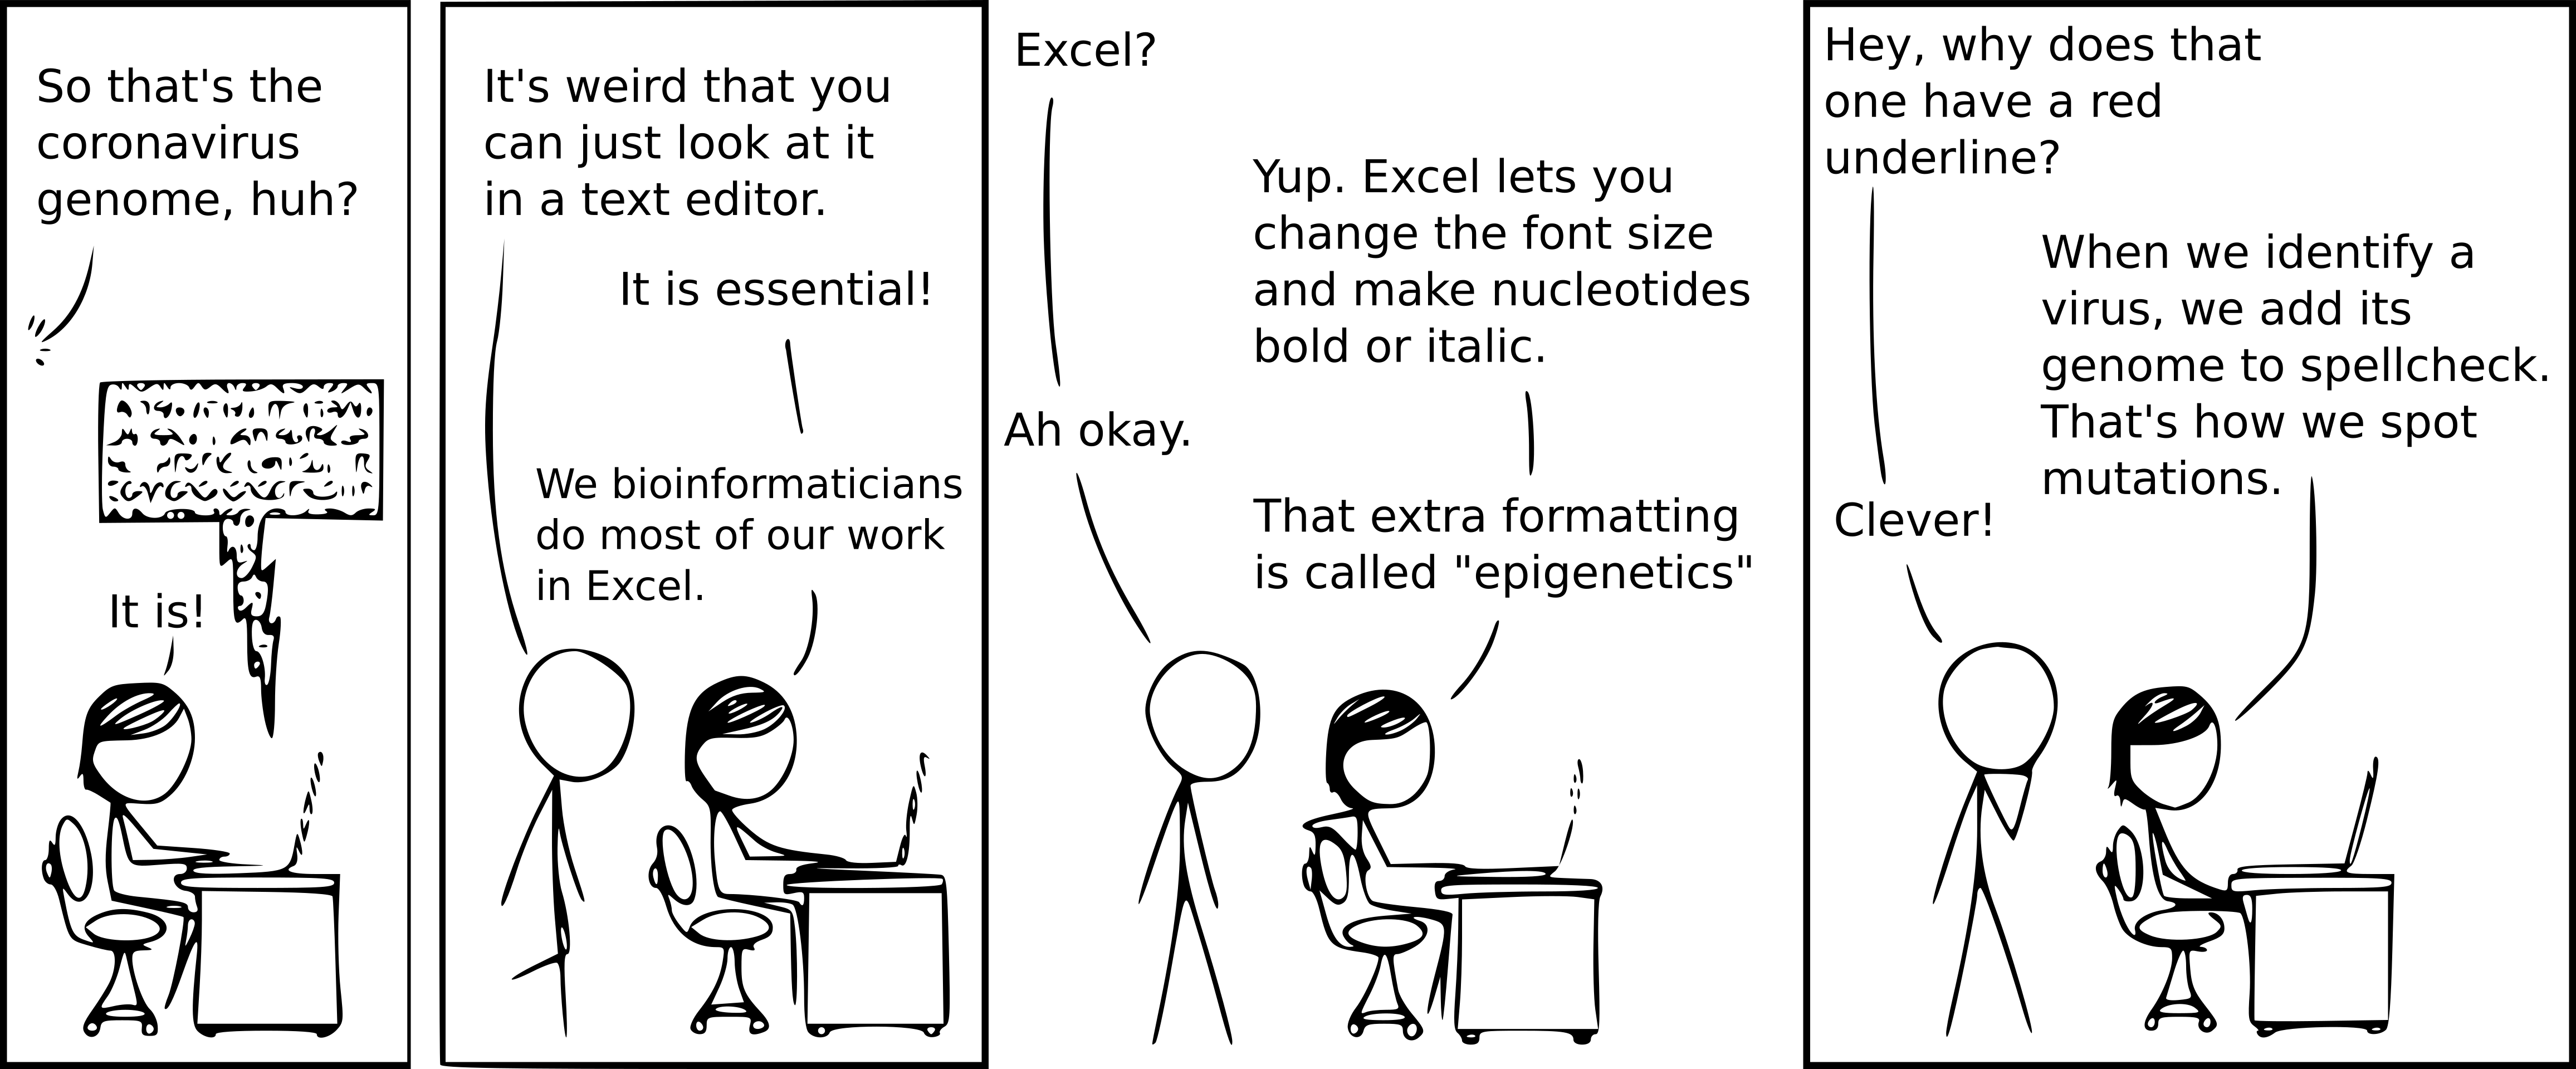
\includegraphics[width=0.85\linewidth]{ch.discussion/imgs/xkcd_excel.png}
    \caption{\textbf{The use of Excel is surprisingly common in bioinformatics.} Adapted from xkcd. URL: https://xkcd.com/2298/}
    \label{fig:xkcd_excel}
\end{figure}

Another part of the problem is that most tools are developed independently, most of the time by a single doctoral student or postdoc. This has two major downsides. The first is that the maintenance of tools depends on individuals. If someone decides to leave academia, their tools, how useful they might be, will soon become obsolete as no one will maintain them. A clear example is the dissolution of the \say{van Heeringen} group, where soon tools such as genomepy\cite{genomepy}, gimmemotifs\cite{Bruse_2018}, ananse\cite{Xu_2020}, scepia, seq2science\cite{seq2science}, and qnorm\cite{qnorm} will become obsolete as they will no longer be maintained. Second, most tools are unnecessarily specialized for the task the developer is trying to solve. This in turn leads to many near-identical implementations that solve the same problem, for example, the many similar SRA-fastq downloading implementations mentioned before, including the seq2science implementation. These problems could be overcome if bioinformaticians would develop more interdepartmental collaborations. A software collaboration between multiple groups and expertise levels would ensure projects are not abandoned when a person leaves and that tools are useful for wider audiences.

In summary, despite the remarkable scientific breakthroughs facilitated by bioinformatics, the field is confronted with an increasingly taxing technical debt. This accumulating technical debt poses challenges for analyses, demanding immediate attention. For a long-term solution to bioinformatics' technical debt, it is necessary to normalize formal training and interdisciplinary collaborations - failure to do so risks inhibiting future advancements in the field.
